\documentclass[12pt]{article}
\pagestyle{plain}
\usepackage[paper=letterpaper,
        left=1in,
        right=1in,
        top=1in,
        bottom=1in] {geometry}
        
\usepackage[parfill]{parskip}
\usepackage{amsmath,amssymb}
\usepackage{tikz}
\usepackage{pgf}
\usepackage{tikz}
\usetikzlibrary{positioning,arrows,automata}
\usepackage[latin1]{inputenc}

\begin{document}
\begin{center}
{\large CS 291}\\
Homework 7
\end{center}

\begin{flushright}
Jingbo Wang\\
jw6347
\end{flushright}
\textbf{Section 11.3, Exercise 3} Suppose we are given the following NFA over the alphabet $\{a, b\}$:

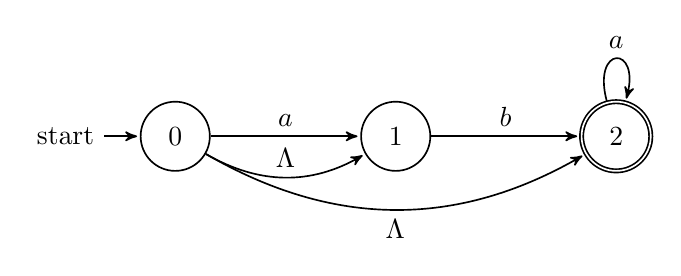
\begin{tikzpicture}[->,>=stealth',shorten >=1pt,auto,node distance=2.8cm,
                    semithick]
  \tikzstyle{every state}=[draw=black,text=black]

  \node[initial,state]            (A)                    {$0$};
  \node[state]                    (B) [right of=A]       {$1$};
  \node[accepting, state]         (C) [right of=B]       {$2$};

  \draw (A) edge [bend right, above] node {$\Lambda$}  (B)
            edge                     node {$a$}        (B)
            edge [below, bend right] node {$\Lambda$}  (C)
        (B) edge                     node {$b$}        (C)
        (C) edge [loop above]        node {$a$}        (C);
\end{tikzpicture}

\textbf{a.} Find a regular expression for the language accepted by the NFA.

\textbf{Answer:}

\begin{center}
\begin{eqnarray*}
\Lambda a^* + (\Lambda + a)ba^*    
& = & \Lambda a^* + (\Lambda ba^* + aba^*) \\
& = & a^* + (ba^* + aba^*) \\
& = & a^* + ba^* + aba^* \\
\end{eqnarray*}
\end{center}

\begin{center}
Therefore, the regular expression for the language accepted by the NFA is $a^* + ba^* + aba^*$. \\
\end{center}

\textbf{b.} Write down the transition table for the NFA.

\textbf{Answer:} 

\begin{center}
\hspace{0.5cm}
\begin{tabular}{cc|cc cc}
           & $T$ & $a$           & $b$           & $\Lambda$     \\
     \cline{2-5}
     Start & $0$ & $\{1\}$       & $\varnothing$ & $\{1, 2\}$    \\
           & $1$ & $\varnothing$ & $\{2\}$       & $\varnothing$ \\
    Final  & $2$ & $\{2\}$       & $\varnothing$ & $\varnothing$ \\
\end{tabular}
\end{center}

\textbf{c.}  Use (11.3.2) to transform the NFA into a DFA.

\textbf{Answer:} 

The first state and final state is $\lambda$(0) = \{0, 1, 2\}. So, we have $T_D$ (\{0, 1, 2\}, a),
and $T_D$(\{0, 1, 2\}, b).\\

\begin{center}
\begin{eqnarray*}
T_D(\{0, 1, 2\}, a)
& = & \lambda(T_N(0,a)\cup T_N(1,a) \cup T_N(2,a)) \\
& = & \lambda(\{1\} \cup \{\varnothing\} \cup \{2\}) \\
& = & \lambda(\{1,2\})\\
& = & \lambda(1) \cup \lambda(2) \\
& = & \{1\} \cup \{2\} \\
& = & \{1, 2\}, \\
\end{eqnarray*}
\end{center}

\begin{center}
\begin{eqnarray*}
T_D(\{0, 1, 2\}, b)
& = & \lambda(T_N(0,b)\cup T_N(1,b) \cup T_N(2,b)) \\
& = & \lambda(\{\varnothing\} \cup \{2\} \cup \{\varnothing\}) \\
& = & \lambda(\{2\})\\
& = & \{2\}. \\
\end{eqnarray*}
\end{center}

The final state are \{1, 2\}, \{2\}. So, we have $T_D$ (\{1, 2\}, a), $T_D$(\{1, 2\}, b), 
$T_D$ (\{2\}, a), and $T_D$ (\{2\}, b).\\

\begin{center}
\begin{eqnarray*}
T_D(\{1, 2\}, a)
& = & \lambda(T_N(1,a) \cup T_N(2,a)) \\
& = & \lambda(\{\varnothing\} \cup \{2\}) \\
& = & \lambda(\{2\})\\
& = & \{2\}, \\
\end{eqnarray*}
\end{center}

\begin{center}
\begin{eqnarray*}
T_D(\{1, 2\}, b)
& = & \lambda(T_N(1,b) \cup T_N(2,b)) \\
& = & \lambda(\{2\} \cup \{\varnothing\}) \\
& = & \lambda(\{2\})\\
& = & \{2\}, \\
\end{eqnarray*}
\end{center}

\begin{center}
\begin{eqnarray*}
T_D(\{2\}, a)
& = & \lambda(T_N(2,a)) \\
& = & \lambda(\{2\}) \\
& = & \{2\}, \\
\end{eqnarray*}
\end{center}

\begin{center}
\begin{eqnarray*}
T_D(\{2\}, b)
& = & \lambda(T_N(2,b)) \\
& = & \lambda(\{\varnothing\}) \\
& = & \varnothing. \\
\end{eqnarray*}
\end{center}

$\varnothing$ is the new enter. So, we have $T_D$ (\{$\varnothing$\}, a) and $T_D$ (\{$\varnothing$\}, b).\\

\begin{center}
\begin{eqnarray*}
T_D(\{\varnothing\}, a)
& = & \lambda(T_N(\varnothing,b)) \\
& = & \lambda(\{\varnothing\}) \\
& = & \varnothing. \\
\end{eqnarray*}
\end{center}

\begin{center}
\begin{eqnarray*}
T_D(\{\varnothing\}, b)
& = & \lambda(T_N(\varnothing,b)) \\
& = & \lambda(\{\varnothing\}) \\
& = & \varnothing. \\
\end{eqnarray*}
\end{center}

Therefore, we have 

\begin{center}
\hspace{0.5cm}
\begin{tabular}{cc|cc}
           & $T$           & $a$           & $b$         \\
     \cline{2-4}
     S   & $\{0, 1, 2\}$ & $\{1,2\}$     & $\{2\}$       \\
     F   & $\{1, 2\}$    & $\{2\}$       & $\{2\}$       \\
     F   & $\{2\}$       & $\{2\}$       & $\varnothing$ \\
         & $\varnothing$ & $\varnothing$ & $\varnothing$ \\
\end{tabular}
\end{center}

$\{0, 1, 2\}$ = 0, $\{1, 2\}$ = 1, $\{2\}$ = 2, $\varnothing$ =3. \\ 
Therefore, we can get

\begin{center}
\hspace{0.5cm}
\begin{tabular}{cc|cc}
           & $T$   & $a$  & $b$ \\
     \cline{2-4}
     S,F   & $0$   & $1$  & $2$ \\
     F     & $1$   & $2$  & $2$ \\
     F     & $2$   & $2$  & $3$ \\
           & $3$   & $3$  & $3$ \\
\end{tabular}
\end{center}

\textbf{d.} Draw a picture of the resulting DFA.

\textbf{Answer:}

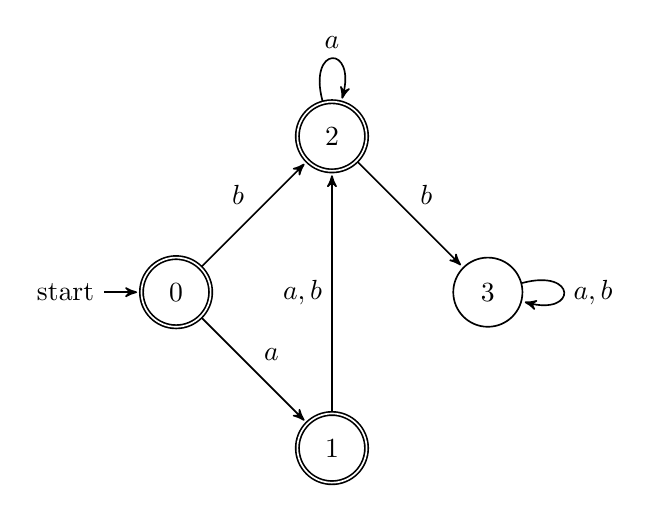
\begin{tikzpicture}[->,>=stealth',shorten >=1pt,auto,node distance=2.8cm,
                    semithick]
  \tikzstyle{every state}=[draw=black,text=black]

  \node[initial,accepting,state]  (A)                    {$0$};
  \node[accepting, state]         (B) [below right of=A] {$1$};
  \node[accepting, state]         (C) [above right of=A] {$2$};
  \node[state]                    (D) [below right of=C] {$3$};
  
  \draw (A) edge                     node {$a$}        (B)
            edge                     node {$b$}        (C)
        (B) edge                     node {$a, b$}     (C)
        (C) edge [loop above]        node {$a$}        (C)
            edge                     node {$b$}        (D)
        (D) edge [loop right]        node {$a,b$}      (D);
\end{tikzpicture}

\textbf{Section 11.4, Exercise 7.b} Show that each of the following languages is not regular by using the
pumping lemma (11.4.3). \\
$\{w | w \in \{a, b\}^* and \enspace w \enspace is \enspace a \enspace palindrome \enspace of \enspace 
even \enspace length\}$.

\textbf{Answer:}

Let \textit{L} = $\{w | w \in \{a, b\}^* and \enspace w \enspace is \enspace a \enspace palindrome \enspace of \enspace 
even \enspace length\}$. \\
Assume, BWOC, the given language is regular. Since w is even length palindrome, we can get 

\begin{center}
s = a$^m$bba$^m$ = xyz, where y $\neq \Lambda$, $|xy| <$ m.   
\end{center}

It follows that x, y is a string of a's, so we can get y = a$^i$, i $>$ 0. If we pump up y to y$^2$, we obtain 

\begin{center}
\begin{eqnarray*}
xy^2z & = & a^ma^ibba^m \\
      & = & a^{m+i}bba^m \\
\end{eqnarray*}
\end{center}

we could easily find that xy$^2 \notin$ \textit{L} because i $>$ 0.\\
Therefore, according to the pumping lemme this language \textit{L} is not regular. \\ 

\textbf{Section 11.5, Exercise 1.a} Find a context-free grammar for each of the following 
languages over the alphabet \{a, b\}.\\

$\{a^nb^{2n} | n \geq 0\}$

\textbf{Answer:}

We can obtain that \{$\Lambda$, abb, aabbbb, aaabbbbbb, ...\}. \\

\begin{center}
$ S \rightarrow \Lambda| aSbb$ \\   
\end{center}

\textbf{Section 11.5, Exercise 2.d}  Find a context-free grammar for each of the following languages. \\
 $\{a^nb^m | n \geq m \geq 0\}$
 
\textbf{Answer:}

We can obtain that \{$\Lambda$, a, ab, aa, aab, aabb, ...\}. \\

\begin{center}
\begin{tabular}{l}
$S \rightarrow aS|aSb|\Lambda$ \\
\end{tabular}
\end{center}
\end{document}
